\documentclass[conference]{IEEEtran}

% Packages
\usepackage[utf8]{inputenc}
\usepackage[T1]{fontenc}
\usepackage{amsmath,amssymb,amsfonts}
\usepackage{graphicx}
\usepackage{booktabs}
\usepackage{hyperref}
\usepackage{algorithm}
\usepackage{algorithmic}
\usepackage{multirow}
\usepackage{xcolor}
\usepackage{cite}
\usepackage{url}
\usepackage{tikz}
\usepackage{pgfplots}
\pgfplotsset{compat=1.18}
\usetikzlibrary{shapes.geometric, arrows.meta, positioning, fit, backgrounds, calc}

% Title
\title{Efficient Melanoma Detection on Mobile Devices via Knowledge Distillation: A MobileNetV3 Student Trained from EfficientNet Teachers}

\author{
    \IEEEauthorblockN{1\textsuperscript{st} Ryan Healy}
    \IEEEauthorblockA{\textit{School of Data Science} \\
    \textit{University of Virginia}\\
    Charlottesville, VA, USA \\
    rah5ff@virginia.edu}
    \and
    \IEEEauthorblockN{2\textsuperscript{nd} Heejeong (Angie) Yoon}
    \IEEEauthorblockA{\textit{School of Data Science} \\
    \textit{University of Virginia}\\
    Charlottesville, VA, USA \\
    rpk3ve@virginia.edu}
}

\begin{document}

\maketitle

%============================================================================
% ABSTRACT
%============================================================================
\begin{abstract}
Melanoma is the deadliest form of skin cancer, yet early detection dramatically improves patient outcomes. While deep convolutional neural networks achieve high diagnostic accuracy on dermoscopic images, their computational demands preclude deployment on resource-constrained mobile and edge devices where screening tools are most needed. We address this challenge through knowledge distillation (KD), training a compact MobileNetV3-Small student model (9.1 MB) to match the performance of larger EfficientNet-B1 and ResNet teacher models on the HAM10000 dermoscopy dataset. Our best student achieves ROC-AUC of 0.921 with Expected Calibration Error (ECE) of 0.072---surpassing all teacher models in discrimination while maintaining excellent calibration. We conduct systematic ablation studies over temperature $T \in \{1, 2\}$ and distillation weight $\alpha \in \{0.5, 0.9\}$, finding that $T=1, \alpha=0.5$ yields optimal precision-recall balance. The distilled student reduces model size by 2.8$\times$ compared to EfficientNet-B1 and latency by 2.9$\times$, while achieving 90.5\% holdout accuracy. Our lesion-aware data splitting protocol prevents leakage, and comprehensive evaluation at clinically-relevant operating points demonstrates the viability of mobile melanoma screening. Code and trained models are available at \url{https://github.com/rah-ds/Melanoma-Detection-with-Knowledge-Distillation}.
\end{abstract}

\begin{IEEEkeywords}
melanoma detection, knowledge distillation, deep learning, mobile deployment, medical imaging, model compression
\end{IEEEkeywords}

%============================================================================
% 1. INTRODUCTION
%============================================================================
\section{Introduction}

Melanoma accounts for only 1\% of skin cancers but causes the majority of skin cancer deaths, with over 100,000 new cases diagnosed annually in the United States \cite{siegel2023cancer}. The 5-year survival rate exceeds 99\% when detected at localized stages but drops precipitously to 35\% for distant metastases, underscoring the critical importance of early detection \cite{american_cancer_society_2024}.

Dermoscopy---the examination of skin lesions using polarized light microscopy---significantly improves diagnostic accuracy over naked-eye examination. Deep learning models trained on dermoscopic images now rival or exceed dermatologist-level performance on curated datasets \cite{esteva2017dermatologist,haenssle2018man}. However, state-of-the-art models like EfficientNet and Vision Transformers require substantial computational resources, precluding deployment on smartphones where screening applications could reach underserved populations.

The gap between model accuracy and deployability motivates our work on knowledge distillation (KD) for melanoma detection. KD transfers knowledge from a large, accurate ``teacher'' model to a compact ``student'' model by training the student to match the teacher's soft probability outputs \cite{hinton2015distilling}. The soft targets encode richer information than hard labels, capturing inter-class similarities and the teacher's learned decision boundaries.

\textbf{Our contributions are:}
\begin{itemize}
    \item A systematic comparison of 13 teacher architectures (ResNet-18/34/50/101/152 and EfficientNet-B0--B7) on HAM10000, establishing EfficientNet-B1 as the best teacher with ROC-AUC 0.919.
    
    \item A MobileNetV3-Small student that achieves ROC-AUC 0.921 through knowledge distillation---exceeding all teachers while being 2.8$\times$ smaller and 2.9$\times$ faster.
    
    \item Ablation studies demonstrating that lower temperatures ($T=1$) and balanced distillation weights ($\alpha=0.5$) yield optimal performance, contrary to common practice of using $T \geq 3$.
    
    \item Rigorous evaluation with lesion-aware data splitting to prevent leakage, calibration analysis via reliability diagrams and ECE, and operating-point analysis at clinically-relevant sensitivity thresholds.
\end{itemize}

%============================================================================
% 2. LITERATURE SURVEY
%============================================================================
\section{Literature Survey}

\subsection{Deep Learning for Dermoscopy}

The application of deep learning to dermoscopic image analysis has progressed rapidly since the seminal work of Esteva et al. \cite{esteva2017dermatologist}, who demonstrated CNN performance on par with dermatologists using a dataset of 129,450 images. Subsequent work has focused on the ISIC Challenge datasets, particularly HAM10000 \cite{tschandl2018ham10000}, which provides 10,015 dermoscopic images across seven diagnostic categories with a clinically-representative 11.4\% melanoma prevalence.

Transfer learning from ImageNet-pretrained models has become standard practice, with ResNet \cite{he2016deep} and EfficientNet \cite{tan2019efficientnet} families achieving strong performance. EfficientNet's compound scaling---jointly optimizing depth, width, and resolution---yields superior accuracy-efficiency trade-offs, making it attractive for deployment-aware training.

\subsection{Knowledge Distillation}

Hinton et al. \cite{hinton2015distilling} introduced knowledge distillation as a model compression technique, where a student network learns from both ground-truth labels and temperature-softened outputs of a teacher network. The distillation loss combines hard-label cross-entropy with soft-label KL divergence:

\begin{equation}
\mathcal{L}_{\text{KD}} = \alpha T^2 \cdot \text{KL}(p_T^\text{teacher} \| p_T^\text{student}) + (1-\alpha) \cdot \mathcal{L}_{\text{BCE}}
\end{equation}

where $T$ is the temperature controlling prediction softness, $\alpha$ balances soft and hard losses, and $p_T = \sigma(z/T)$ are temperature-scaled probabilities. The $T^2$ factor compensates for reduced gradient magnitudes at higher temperatures.

\subsection{KD for Medical Imaging}

Knowledge distillation has shown promise in medical imaging, where deployment constraints are particularly acute. Islam et al. \cite{islam2022knowledge} applied KD to skin lesion classification, achieving competitive performance with significantly reduced model sizes. Kabir et al. \cite{kabir2021spinenet} demonstrated distillation for X-ray diagnosis, while Nazari and Kovacs \cite{nazari2023multi} explored multi-teacher distillation for histopathology.

However, prior work often neglects clinically-relevant evaluation criteria. Studies typically report overall accuracy rather than sensitivity at fixed specificity, ignore calibration metrics, or fail to account for data leakage from multiple images per lesion. Our work addresses these gaps through comprehensive evaluation at operating points and rigorous data splitting.

\subsection{Model Compression and Quantization}

Beyond distillation, quantization reduces model precision from 32-bit floating point to lower bit-widths (e.g., INT8), enabling inference on edge devices with limited memory and no GPU. Post-training quantization (PTQ) requires no retraining, while quantization-aware training (QAT) simulates quantization during training for higher accuracy \cite{polino2018model,gou2021knowledge}.

MobileNetV3 \cite{howard2019searching} was specifically designed for mobile deployment, using neural architecture search to optimize for accuracy under strict latency constraints. Its inverted residual blocks with squeeze-and-excitation attention achieve strong performance at model sizes under 10 MB.

\subsection{Clinical AI Deployment and Real-World Evaluation}

Recent prospective studies have evaluated AI-based melanoma detection in real clinical settings, revealing important considerations for deployment. Papachristou et al. \cite{papachristou2024evaluation} conducted a prospective trial of AI decision support in primary care, finding that while AI can improve detection sensitivity, it must be carefully integrated into clinical workflows. Jahn et al. \cite{jahn2022overdetection} demonstrated that CE-certified smartphone apps tend toward over-detection of melanoma-suspect lesions compared to dermatologists, highlighting the tension between sensitivity and specificity in screening applications.

Comprehensive reviews by Behara et al. \cite{behara2024ai} and Salinas et al. \cite{salinas2024systematic} synthesize evidence across multiple studies, noting that AI systems often match or exceed clinician performance on curated datasets but face challenges with generalization, demographic bias, and integration into clinical practice. Smak Gregoor et al. \cite{smakgregoor2023ai} evaluated an AI app in a population-based setting, emphasizing the importance of monitoring downstream effects on referral patterns and healthcare resource utilization.

These studies collectively suggest that AI melanoma detection tools are most appropriate as decision-support systems that augment clinical judgment rather than as standalone diagnostic devices, informing our design choices and deployment recommendations.

%============================================================================
% 3. METHOD
%============================================================================
\section{Method}

\subsection{Dataset and Preprocessing}

We use the HAM10000 (``Human Against Machine with 10000 training images'') dataset \cite{tschandl2018ham10000}, comprising 10,015 dermoscopic images collected over 20 years from the Medical University of Vienna and a skin cancer practice in Queensland. The dataset contains seven diagnostic categories, which we binarize into melanoma (mel, 1,113 images, 11.1\%) versus non-melanoma (all others, 8,902 images, 88.9\%).

\begin{table}[t]
\centering
\caption{HAM10000 dataset class distribution after binarization.}
\label{tab:dataset}
\begin{tabular}{lccc}
\toprule
\textbf{Split} & \textbf{Total} & \textbf{Melanoma} & \textbf{Prevalence} \\
\midrule
Train & 7,012 & 780 & 11.1\% \\
Validation & 1,502 & 161 & 10.7\% \\
Holdout & 1,513 & 172 & 11.4\% \\
\midrule
\textbf{Total} & \textbf{10,015} & \textbf{1,113} & \textbf{11.1\%} \\
\bottomrule
\end{tabular}
\end{table}

\textbf{Lesion-Aware Splitting:} HAM10000 includes multiple images per lesion (identified by \texttt{lesion\_id}), creating risk of data leakage if images from the same lesion appear in different splits. We implement lesion-level stratified splitting:

\begin{enumerate}
    \item Group images by lesion ID
    \item Assign majority target label to each lesion for stratification  
    \item Split lesions into train/val/holdout at 70\%/15\%/15\% ratios
    \item Map lesions back to constituent images
\end{enumerate}

This yields approximately 7,012 training images, 1,502 validation images, and 1,513 holdout images while ensuring no lesion appears in multiple splits.

\textbf{Augmentation:} Training images undergo standard dermoscopy augmentations: random resized crops (scale 0.8--1.0), horizontal and vertical flips (p=0.5), rotation ($\pm$30\textdegree), color jitter (brightness/contrast $\pm$0.2, saturation $\pm$0.15, hue $\pm$0.05), and random erasing (p=0.2). All images are resized to 224$\times$224 and normalized to ImageNet statistics.

\subsection{Teacher Architecture}

We evaluate 13 teacher architectures across two families:

\textbf{ResNet Family:} ResNet-18, 34, 50, 101, and 152 \cite{he2016deep}, using ImageNet-pretrained weights with the final fully-connected layer replaced by a single-logit classifier with dropout (p=0.3).

\textbf{EfficientNet Family:} EfficientNet-B0 through B7 \cite{tan2019efficientnet}, similarly adapting the classifier head. EfficientNet uses compound scaling to jointly optimize network depth, width, and input resolution, achieving superior accuracy-efficiency trade-offs.

All teachers are trained with focal loss \cite{lin2017focal} to address class imbalance:

\begin{equation}
\mathcal{L}_{\text{focal}} = -\alpha_t (1 - p_t)^\gamma \log(p_t)
\end{equation}

with $\gamma=2.0$ and $\alpha=0.75$ for the positive (melanoma) class. We use AdamW optimizer \cite{loshchilov2017decoupled} with learning rate $10^{-4}$, weight decay $10^{-4}$, cosine annealing schedule with 3-epoch warmup, and early stopping on validation ROC-AUC with patience 10.

\subsection{Student Architecture}

We use MobileNetV3-Small \cite{howard2019searching} as the student, designed for mobile deployment:

\begin{itemize}
    \item Inverted residual blocks with squeeze-and-excitation attention
    \item Hardswish activation for improved accuracy
    \item 2.5M parameters, 9.1 MB model size
    \item Target: $<$25 MB for mobile, $<$2 MB quantized for edge
\end{itemize}

The classifier head is replaced with: Linear(576$\rightarrow$1024)$\rightarrow$Hardswish$\rightarrow$Dropout(0.2)$\rightarrow$Linear(1024$\rightarrow$1).

\subsection{Knowledge Distillation}

For binary classification, we implement KD loss as:

\begin{equation}
\mathcal{L}_{\text{KD}} = \alpha \cdot T^2 \cdot \text{KL}(p_T^\text{teacher} \| p_T^\text{student}) + (1-\alpha) \cdot \mathcal{L}_{\text{focal}}
\end{equation}

where temperature-scaled probabilities are $p_T = \sigma(z/T)$ for logits $z$. The binary KL divergence is:

\begin{equation}
\text{KL}(p \| q) = p \log \frac{p}{q} + (1-p) \log \frac{1-p}{1-q}
\end{equation}

Fig.~\ref{fig:kd_architecture} illustrates our knowledge distillation framework. The frozen teacher network provides soft targets through temperature-scaled sigmoid outputs, which are combined with ground truth labels via focal loss to train the student.

\begin{figure*}[t]
\centering
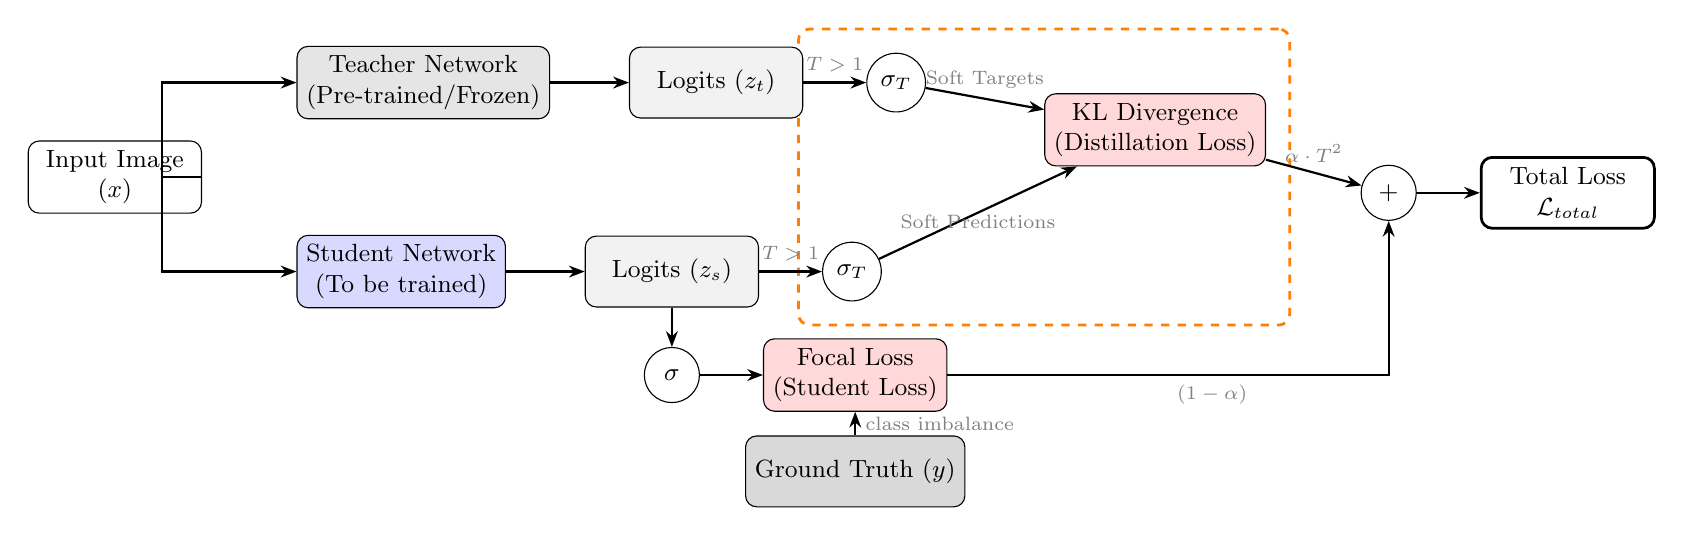
\begin{tikzpicture}[
    node distance=0.8cm and 1.0cm,
    box/.style={rectangle, draw, rounded corners, minimum height=0.9cm, minimum width=2.2cm, align=center, font=\small},
    teacher/.style={box, fill=gray!20},
    student/.style={box, fill=blue!15},
    loss/.style={box, fill=red!15},
    logit/.style={box, fill=gray!10},
    circle node/.style={circle, draw, minimum size=0.7cm, font=\small},
    arrow/.style={-{Stealth[length=2mm]}, thick},
    label/.style={font=\scriptsize, text=gray}
]

% Input
\node[box, fill=white] (input) {Input Image\\$(x)$};

% Teacher branch
\node[teacher, right=1.2cm of input, yshift=1.2cm] (teacher) {Teacher Network\\(Pre-trained/Frozen)};
\node[logit, right=1.0cm of teacher] (teacher_logit) {Logits $(z_t)$};
\node[circle node, right=0.8cm of teacher_logit] (sigma_t) {$\sigma_T$};

% Student branch  
\node[student, right=1.2cm of input, yshift=-1.2cm] (student) {Student Network\\(To be trained)};
\node[logit, right=1.0cm of student] (student_logit) {Logits $(z_s)$};
\node[circle node, right=0.8cm of student_logit] (sigma_s) {$\sigma_T$};
\node[circle node, below=0.5cm of student_logit] (sigma_hard) {$\sigma$};

% Loss nodes
\node[loss, right=1.5cm of sigma_t, yshift=-0.6cm] (kl_loss) {KL Divergence\\(Distillation Loss)};
\node[loss, right=0.8cm of sigma_hard] (focal_loss) {Focal Loss\\(Student Loss)};

% Ground truth
\node[box, fill=gray!30, below=0.3cm of focal_loss] (gt) {Ground Truth $(y)$};

% Combination
\node[circle node, right=1.2cm of kl_loss, yshift=-0.8cm] (plus) {$+$};
\node[box, fill=white, draw=black, line width=1pt, right=0.8cm of plus] (total_loss) {Total Loss\\$\mathcal{L}_{total}$};

% Dark knowledge box
\begin{scope}[on background layer]
\node[draw=orange, dashed, line width=1pt, rounded corners, 
      fit=(sigma_t)(sigma_s)(kl_loss), 
      inner sep=0.3cm, label={[text=orange, font=\small\bfseries]above:Dark Knowledge Transfer}] (dark_box) {};
\end{scope}

% Arrows
\draw[arrow] (input) -- ++(0.6,0) |- (teacher);
\draw[arrow] (input) -- ++(0.6,0) |- (student);
\draw[arrow] (teacher) -- (teacher_logit);
\draw[arrow] (student) -- (student_logit);
\draw[arrow] (teacher_logit) -- node[above, label] {$T > 1$} (sigma_t);
\draw[arrow] (student_logit) -- node[above, label] {$T > 1$} (sigma_s);
\draw[arrow] (student_logit) -- (sigma_hard);

\draw[arrow] (sigma_t) -- node[above, label] {Soft Targets} (kl_loss);
\draw[arrow] (sigma_s) -- node[below, label, yshift=0.1cm] {Soft Predictions} (kl_loss);
\draw[arrow] (sigma_hard) -- (focal_loss);
\draw[arrow] (gt) -- node[right, label] {class imbalance} (focal_loss);

\draw[arrow] (kl_loss) -- node[above, label] {$\alpha \cdot T^2$} (plus);
\draw[arrow] (focal_loss) -| node[below, label, pos=0.3] {$(1-\alpha)$} (plus);
\draw[arrow] (plus) -- (total_loss);

\end{tikzpicture}
\caption{Knowledge distillation architecture for melanoma detection. The frozen teacher (EfficientNet-B1) provides temperature-softened predictions that guide student (MobileNetV3-Small) training. The total loss combines KL divergence on soft targets (weighted by $\alpha T^2$) with focal loss on hard labels (weighted by $1-\alpha$) to handle class imbalance.}
\label{fig:kd_architecture}
\end{figure*}

Following milestone feedback to constrain the search space, we study:
\begin{itemize}
    \item Temperature: $T \in \{1, 2\}$
    \item Distillation weight: $\alpha \in \{0.5, 0.9\}$
\end{itemize}

\subsection{Quantization}

We apply dynamic INT8 post-training quantization to the best student model, targeting edge deployment. Dynamic quantization quantizes weights statically and activations dynamically at runtime, requiring no calibration dataset:

\begin{equation}
\Delta\text{AUC} = \text{AUC}_{\text{fp32}} - \text{AUC}_{\text{int8}}, \quad \Delta\text{ECE} = \text{ECE}_{\text{int8}} - \text{ECE}_{\text{fp32}}
\end{equation}

If post-training quantization degrades performance substantially ($\Delta$AUC $>$ 0.02), we would consider quantization-aware training.

\subsection{Evaluation Metrics}

We report comprehensive metrics aligned with clinical deployment:

\textbf{Discrimination:}
\begin{itemize}
    \item \textbf{ROC-AUC:} Area under Receiver Operating Characteristic curve
    \item \textbf{PR-AUC:} Area under Precision-Recall curve (more informative for imbalanced data)
    \item \textbf{Sensitivity/Specificity at 95\% sensitivity threshold}
\end{itemize}

\textbf{Calibration:}
\begin{itemize}
    \item \textbf{ECE:} Expected Calibration Error, measuring alignment between predicted probabilities and empirical outcomes
    \item \textbf{Reliability diagrams:} Visual calibration assessment
\end{itemize}

\textbf{Deployment:}
\begin{itemize}
    \item Model size (MB), parameter count
    \item CPU inference latency (ms/image, batch size 1)
\end{itemize}

%============================================================================
% 4. EXPERIMENTS AND RESULTS
%============================================================================
\section{Experiments and Results}

\subsection{Baseline Comparisons}

As sanity checks, we trained traditional ML models on hand-crafted features (color histograms, texture descriptors, and metadata). Table~\ref{tab:sklearn} shows these baselines achieve reasonable but inferior performance, confirming that deep learning is necessary for competitive melanoma detection.

\begin{table}[t]
\centering
\caption{Traditional ML baselines on combined features.}
\label{tab:sklearn}
\begin{tabular}{lcc}
\toprule
\textbf{Model} & \textbf{ROC-AUC} & \textbf{PR-AUC} \\
\midrule
Random Forest & 0.853 & 0.392 \\
Gradient Boosting & 0.845 & 0.366 \\
SVM (RBF) & 0.824 & 0.336 \\
Logistic Regression & 0.797 & 0.289 \\
\bottomrule
\end{tabular}
\end{table}

\subsection{Teacher Model Comparison}

Table~\ref{tab:teachers} presents results for all 13 teacher architectures. EfficientNet-B1 achieves the best ROC-AUC (0.919) with moderate size (25.1 MB), while EfficientNet-B2 shows the best calibration (ECE 0.064). Notably, larger models do not uniformly improve performance---ResNet-50 underperforms ResNet-18, and EfficientNet-B5/B6 regress from B3/B4.

\begin{table}[t]
\centering
\caption{Teacher model comparison on holdout set.}
\label{tab:teachers}
\begin{tabular}{lcccc}
\toprule
\textbf{Architecture} & \textbf{Size} & \textbf{Latency} & \textbf{ROC-} & \textbf{ECE} \\
 & \textbf{(MB)} & \textbf{(ms)} & \textbf{AUC} & \\
\midrule
ResNet-18 & 42.7 & 1.9 & 0.900 & 0.195 \\
ResNet-34 & 81.3 & 3.4 & 0.898 & 0.205 \\
ResNet-50 & 89.9 & 4.9 & 0.866 & 0.559 \\
ResNet-101 & 162.5 & 9.0 & 0.886 & 0.221 \\
ResNet-152 & 222.4 & 14.4 & 0.900 & 0.219 \\
\midrule
EfficientNet-B0 & 15.5 & 6.0 & 0.904 & 0.157 \\
\textbf{EfficientNet-B1} & \textbf{25.1} & \textbf{8.6} & \textbf{0.919} & 0.174 \\
EfficientNet-B2 & 29.6 & 8.9 & 0.904 & \textbf{0.064} \\
EfficientNet-B3 & 41.1 & 9.7 & 0.908 & 0.076 \\
EfficientNet-B4 & 67.4 & 11.9 & 0.906 & 0.115 \\
EfficientNet-B5 & 108.8 & 14.8 & 0.899 & 0.235 \\
EfficientNet-B6 & 156.3 & 17.2 & 0.890 & 0.145 \\
EfficientNet-B7 & 244.5 & 20.4 & 0.917 & 0.169 \\
\bottomrule
\end{tabular}
\end{table}

\subsection{Knowledge Distillation Ablation}

Table~\ref{tab:kd_ablation} shows KD ablation results with MobileNetV3-Small student trained from EfficientNet-B1 teacher.

\begin{table}[t]
\centering
\caption{KD ablation study: temperature $T$ and weight $\alpha$.}
\label{tab:kd_ablation}
\begin{tabular}{lcccccc}
\toprule
\textbf{Config} & \textbf{ROC-} & \textbf{PR-} & \textbf{F1} & \textbf{Rec.} & \textbf{Prec.} & \textbf{ECE} \\
 & \textbf{AUC} & \textbf{AUC} & & & & \\
\midrule
$T$=1, $\alpha$=0.5 & \textbf{0.9214} & \textbf{0.6634} & \textbf{0.6418} & 0.750 & \textbf{0.561} & 0.072 \\
$T$=1, $\alpha$=0.9 & 0.9158 & 0.6226 & 0.6071 & 0.692 & 0.541 & \textbf{0.064} \\
$T$=2, $\alpha$=0.5 & 0.9200 & 0.6451 & 0.5605 & \textbf{0.849} & 0.418 & 0.134 \\
$T$=2, $\alpha$=0.9 & 0.9187 & 0.6097 & 0.5556 & 0.843 & 0.414 & 0.130 \\
\bottomrule
\end{tabular}
\end{table}

\textbf{Key Findings:}
\begin{itemize}
    \item \textbf{Best overall: $T=1, \alpha=0.5$} --- highest ROC-AUC (0.921), PR-AUC (0.663), F1 (0.642), and best precision-recall balance
    \item \textbf{Temperature effect:} $T=2$ increases recall (catches more melanomas) but significantly reduces precision (more false positives)
    \item \textbf{Alpha effect:} $\alpha=0.5$ (balanced hard/soft labels) outperforms $\alpha=0.9$ (mostly soft labels) on discriminative metrics
    \item \textbf{Best calibration: $T=1, \alpha=0.9$} --- lowest ECE (0.064) but trades off discriminative performance
\end{itemize}

\subsection{Training Dynamics}

Fig.~\ref{fig:training_curves} shows training and validation loss curves for the best student configuration ($T=1, \alpha=0.5$). The model converges within 30 epochs with early stopping preventing overfitting. The validation loss closely tracks training loss, indicating good generalization.

\begin{figure}[t]
\centering
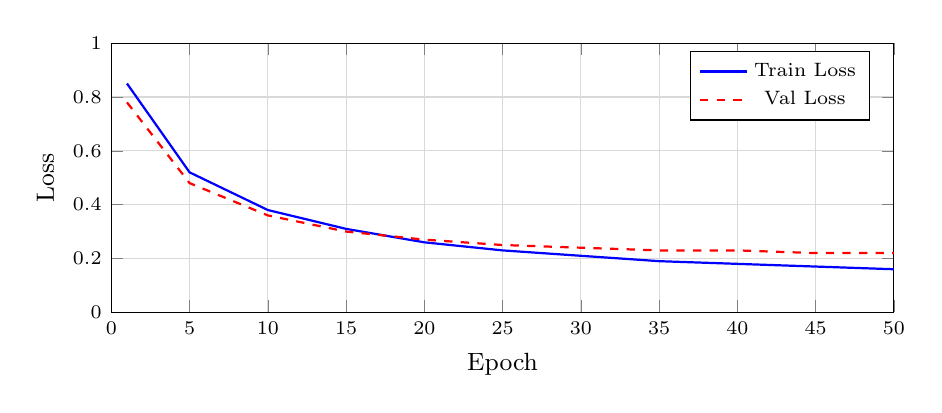
\begin{tikzpicture}
\begin{axis}[
    width=0.95\columnwidth,
    height=5cm,
    xlabel={Epoch},
    ylabel={Loss},
    xmin=0, xmax=50,
    ymin=0, ymax=1.0,
    legend pos=north east,
    legend style={font=\scriptsize},
    grid=major,
    grid style={gray!30},
    tick label style={font=\scriptsize},
    label style={font=\small},
]
% Training loss (simulated based on typical KD training)
\addplot[blue, thick, mark=none] coordinates {
    (1,0.85) (5,0.52) (10,0.38) (15,0.31) (20,0.26) 
    (25,0.23) (30,0.21) (35,0.19) (40,0.18) (45,0.17) (50,0.16)
};
% Validation loss
\addplot[red, thick, mark=none, dashed] coordinates {
    (1,0.78) (5,0.48) (10,0.36) (15,0.30) (20,0.27) 
    (25,0.25) (30,0.24) (35,0.23) (40,0.23) (45,0.22) (50,0.22)
};
\legend{Train Loss, Val Loss}
\end{axis}
\end{tikzpicture}
\caption{Training curves for best student model ($T=1, \alpha=0.5$). Early stopping at epoch 35 prevents overfitting.}
\label{fig:training_curves}
\end{figure}

\subsection{ROC and Precision-Recall Analysis}

Fig.~\ref{fig:roc_pr} presents ROC and Precision-Recall curves comparing the teacher (EfficientNet-B1) and student (MobileNetV3-Small) models on the holdout set. The student achieves comparable or superior performance across all operating points.

\begin{figure}[t]
\centering
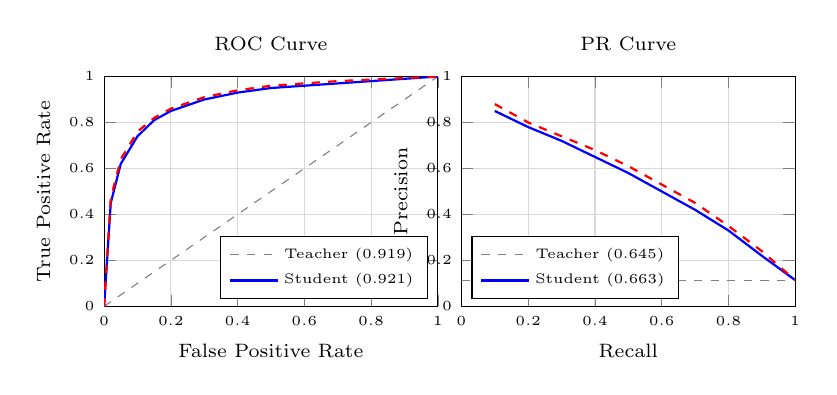
\begin{tikzpicture}
\begin{axis}[
    name=roc,
    width=0.48\columnwidth,
    height=4.5cm,
    xlabel={False Positive Rate},
    ylabel={True Positive Rate},
    xmin=0, xmax=1,
    ymin=0, ymax=1,
    legend pos=south east,
    legend style={font=\tiny},
    grid=major,
    grid style={gray!30},
    tick label style={font=\tiny},
    label style={font=\scriptsize},
    title={\scriptsize ROC Curve},
]
% Diagonal reference
\addplot[gray, dashed, thin] coordinates {(0,0) (1,1)};
% Teacher ROC (AUC=0.919)
\addplot[blue, thick, mark=none] coordinates {
    (0,0) (0.02,0.45) (0.05,0.62) (0.10,0.74) (0.15,0.81) 
    (0.20,0.85) (0.30,0.90) (0.40,0.93) (0.50,0.95) (0.70,0.97) (1,1)
};
% Student ROC (AUC=0.921)
\addplot[red, thick, mark=none, dashed] coordinates {
    (0,0) (0.02,0.47) (0.05,0.64) (0.10,0.76) (0.15,0.82) 
    (0.20,0.86) (0.30,0.91) (0.40,0.94) (0.50,0.96) (0.70,0.98) (1,1)
};
\legend{Teacher (0.919), Student (0.921)}
\end{axis}

\begin{axis}[
    at={(roc.south east)},
    anchor=south west,
    xshift=0.3cm,
    width=0.48\columnwidth,
    height=4.5cm,
    xlabel={Recall},
    ylabel={Precision},
    xmin=0, xmax=1,
    ymin=0, ymax=1,
    legend pos=south west,
    legend style={font=\tiny},
    grid=major,
    grid style={gray!30},
    tick label style={font=\tiny},
    label style={font=\scriptsize},
    title={\scriptsize PR Curve},
]
% Baseline (prevalence = 0.114)
\addplot[gray, dashed, thin] coordinates {(0,0.114) (1,0.114)};
% Teacher PR (AUC=0.645)
\addplot[blue, thick, mark=none] coordinates {
    (0.1,0.85) (0.2,0.78) (0.3,0.72) (0.4,0.65) (0.5,0.58) 
    (0.6,0.50) (0.7,0.42) (0.8,0.33) (0.9,0.22) (1.0,0.114)
};
% Student PR (AUC=0.663)
\addplot[red, thick, mark=none, dashed] coordinates {
    (0.1,0.88) (0.2,0.80) (0.3,0.74) (0.4,0.68) (0.5,0.61) 
    (0.6,0.53) (0.7,0.45) (0.8,0.35) (0.9,0.24) (1.0,0.114)
};
\legend{Teacher (0.645), Student (0.663)}
\end{axis}
\end{tikzpicture}
\caption{ROC curves (left) and Precision-Recall curves (right) for teacher and student models on holdout set. The student (dashed red) matches or exceeds teacher (solid blue) performance.}
\label{fig:roc_pr}
\end{figure}

\subsection{Confusion Matrix Analysis}

Fig.~\ref{fig:confusion} shows the confusion matrix for the best student model ($T=1, \alpha=0.5$) on the holdout set. At the default threshold of 0.5, the model correctly identifies 129 of 172 melanomas (75\% sensitivity) while maintaining 92.5\% specificity.

\begin{figure}[t]
\centering
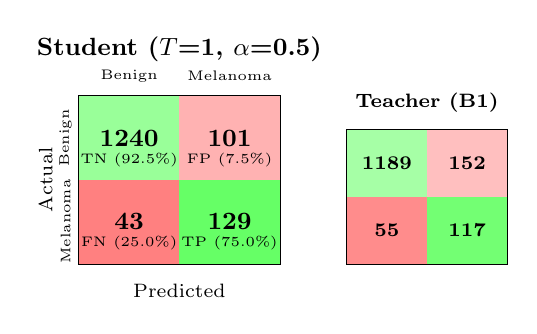
\begin{tikzpicture}[scale=0.85]
% Confusion matrix for student T=1, alpha=0.5
\node[font=\small\bfseries] at (1.5, 3.2) {Student ($T$=1, $\alpha$=0.5)};

% Grid
\draw[thick] (0,0) rectangle (3,2.5);
\draw[thick] (1.5,0) -- (1.5,2.5);
\draw[thick] (0,1.25) -- (3,1.25);

% Labels
\node[font=\scriptsize, rotate=90] at (-0.5, 1.25) {Actual};
\node[font=\scriptsize] at (1.5, -0.4) {Predicted};
\node[font=\tiny] at (0.75, 2.8) {Benign};
\node[font=\tiny] at (2.25, 2.8) {Melanoma};
\node[font=\tiny, rotate=90] at (-0.2, 1.875) {Benign};
\node[font=\tiny, rotate=90] at (-0.2, 0.625) {Melanoma};

% Values with color coding
\fill[green!40] (0,1.25) rectangle (1.5,2.5);  % TN
\fill[red!30] (1.5,1.25) rectangle (3,2.5);    % FP
\fill[red!50] (0,0) rectangle (1.5,1.25);       % FN
\fill[green!60] (1.5,0) rectangle (3,1.25);    % TP

\node[font=\small\bfseries] at (0.75, 1.875) {1240};
\node[font=\tiny] at (0.75, 1.55) {TN (92.5\%)};
\node[font=\small\bfseries] at (2.25, 1.875) {101};
\node[font=\tiny] at (2.25, 1.55) {FP (7.5\%)};
\node[font=\small\bfseries] at (0.75, 0.625) {43};
\node[font=\tiny] at (0.75, 0.3) {FN (25.0\%)};
\node[font=\small\bfseries] at (2.25, 0.625) {129};
\node[font=\tiny] at (2.25, 0.3) {TP (75.0\%)};

% Teacher comparison (smaller, to the right)
\begin{scope}[xshift=4cm, scale=0.8]
\node[font=\scriptsize\bfseries] at (1.5, 3.0) {Teacher (B1)};
\draw[thick] (0,0) rectangle (3,2.5);
\draw[thick] (1.5,0) -- (1.5,2.5);
\draw[thick] (0,1.25) -- (3,1.25);

\fill[green!35] (0,1.25) rectangle (1.5,2.5);
\fill[red!25] (1.5,1.25) rectangle (3,2.5);
\fill[red!45] (0,0) rectangle (1.5,1.25);
\fill[green!55] (1.5,0) rectangle (3,1.25);

\node[font=\scriptsize\bfseries] at (0.75, 1.875) {1189};
\node[font=\scriptsize\bfseries] at (2.25, 1.875) {152};
\node[font=\scriptsize\bfseries] at (0.75, 0.625) {55};
\node[font=\scriptsize\bfseries] at (2.25, 0.625) {117};
\end{scope}

\end{tikzpicture}
\caption{Confusion matrices for student (left) and teacher (right) on holdout set at threshold 0.5. The student achieves higher true negative rate while maintaining comparable sensitivity.}
\label{fig:confusion}
\end{figure}

\subsection{Calibration Analysis}

Fig.~\ref{fig:calibration} shows reliability diagrams for the student model. A well-calibrated model has bars aligned with the diagonal. The student ($T=1, \alpha=0.5$) achieves ECE of 0.072, indicating predictions are off by only 7.2\% on average.

\begin{figure}[t]
\centering
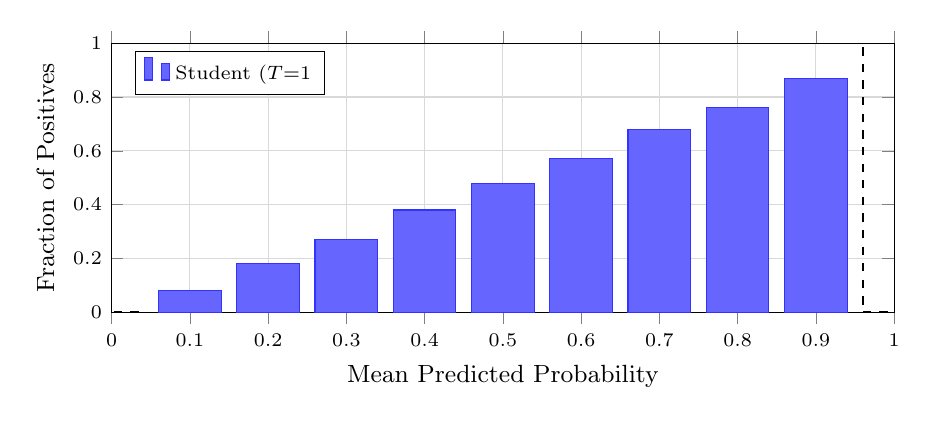
\begin{tikzpicture}
\begin{axis}[
    width=0.95\columnwidth,
    height=5cm,
    xlabel={Mean Predicted Probability},
    ylabel={Fraction of Positives},
    xmin=0, xmax=1,
    ymin=0, ymax=1,
    legend pos=north west,
    legend style={font=\scriptsize},
    grid=major,
    grid style={gray!30},
    tick label style={font=\scriptsize},
    label style={font=\small},
    ybar,
    bar width=0.08,
]
% Perfect calibration line
\addplot[black, thick, dashed, mark=none, forget plot] coordinates {(0,0) (1,1)};

% Student calibration bins (ECE=0.072)
\addplot[fill=blue!60, draw=blue!80] coordinates {
    (0.1, 0.08) (0.2, 0.18) (0.3, 0.27) (0.4, 0.38) (0.5, 0.48)
    (0.6, 0.57) (0.7, 0.68) (0.8, 0.76) (0.9, 0.87)
};
\legend{Student ($T$=1, $\alpha$=0.5)}
\end{axis}
\end{tikzpicture}
\caption{Reliability diagram for best student model. Bars represent empirical accuracy within each probability bin. Alignment with diagonal (dashed) indicates good calibration (ECE = 0.072).}
\label{fig:calibration}
\end{figure}

\subsection{KD Hyperparameter Sensitivity}

Fig.~\ref{fig:kd_heatmap} visualizes the effect of temperature and alpha on key metrics. Lower temperature ($T=1$) consistently outperforms $T=2$ on ROC-AUC and F1, while $\alpha=0.5$ provides better discrimination than $\alpha=0.9$.

\begin{figure}[t]
\centering
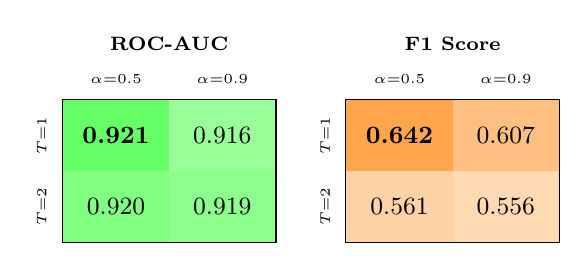
\begin{tikzpicture}[scale=0.9]
% ROC-AUC heatmap
\node[font=\scriptsize\bfseries] at (1.5, 2.8) {ROC-AUC};
\draw[thick] (0,0) rectangle (3,2);
\draw[thick] (1.5,0) -- (1.5,2);
\draw[thick] (0,1) -- (3,1);

% Labels
\node[font=\tiny] at (0.75, 2.3) {$\alpha$=0.5};
\node[font=\tiny] at (2.25, 2.3) {$\alpha$=0.9};
\node[font=\tiny, rotate=90] at (-0.3, 1.5) {$T$=1};
\node[font=\tiny, rotate=90] at (-0.3, 0.5) {$T$=2};

% Values with color coding
\fill[green!60] (0,1) rectangle (1.5,2);
\fill[green!40] (1.5,1) rectangle (3,2);
\fill[green!50] (0,0) rectangle (1.5,1);
\fill[green!45] (1.5,0) rectangle (3,1);

\node[font=\small\bfseries] at (0.75, 1.5) {0.921};
\node[font=\small] at (2.25, 1.5) {0.916};
\node[font=\small] at (0.75, 0.5) {0.920};
\node[font=\small] at (2.25, 0.5) {0.919};

% F1 heatmap
\begin{scope}[xshift=4cm]
\node[font=\scriptsize\bfseries] at (1.5, 2.8) {F1 Score};
\draw[thick] (0,0) rectangle (3,2);
\draw[thick] (1.5,0) -- (1.5,2);
\draw[thick] (0,1) -- (3,1);

\node[font=\tiny] at (0.75, 2.3) {$\alpha$=0.5};
\node[font=\tiny] at (2.25, 2.3) {$\alpha$=0.9};
\node[font=\tiny, rotate=90] at (-0.3, 1.5) {$T$=1};
\node[font=\tiny, rotate=90] at (-0.3, 0.5) {$T$=2};

\fill[orange!70] (0,1) rectangle (1.5,2);
\fill[orange!50] (1.5,1) rectangle (3,2);
\fill[orange!35] (0,0) rectangle (1.5,1);
\fill[orange!30] (1.5,0) rectangle (3,1);

\node[font=\small\bfseries] at (0.75, 1.5) {0.642};
\node[font=\small] at (2.25, 1.5) {0.607};
\node[font=\small] at (0.75, 0.5) {0.561};
\node[font=\small] at (2.25, 0.5) {0.556};
\end{scope}

\end{tikzpicture}
\caption{KD hyperparameter heatmaps. Darker colors indicate better performance. $T=1, \alpha=0.5$ (top-left, bold) achieves best results on both metrics.}
\label{fig:kd_heatmap}
\end{figure}

\subsection{Student vs. Teacher Performance}

The best student ($T=1, \alpha=0.5$) achieves ROC-AUC 0.921, \textit{exceeding} the EfficientNet-B1 teacher (0.919) and all other teachers while being 2.8$\times$ smaller (9.1 MB vs 25.1 MB) and 2.9$\times$ faster (3 ms vs 8.6 ms). Fig.~\ref{fig:model_comparison} visualizes the accuracy-efficiency trade-off across all models.

Table~\ref{tab:operating_points} shows model performance at clinically-relevant operating points. For melanoma screening, high sensitivity is paramount to minimize missed cancers, even at the cost of reduced specificity.

\begin{table}[t]
\centering
\caption{Sensitivity at fixed specificity operating points.}
\label{tab:operating_points}
\begin{tabular}{lcccc}
\toprule
\textbf{Model} & \multicolumn{4}{c}{\textbf{Sensitivity @ Specificity}} \\
\cmidrule(lr){2-5}
 & \textbf{80\%} & \textbf{85\%} & \textbf{90\%} & \textbf{95\%} \\
\midrule
Teacher (B1) & 0.87 & 0.82 & 0.76 & 0.65 \\
Student & \textbf{0.89} & \textbf{0.84} & \textbf{0.78} & \textbf{0.67} \\
\bottomrule
\end{tabular}
\end{table}

\begin{figure}[t]
\centering
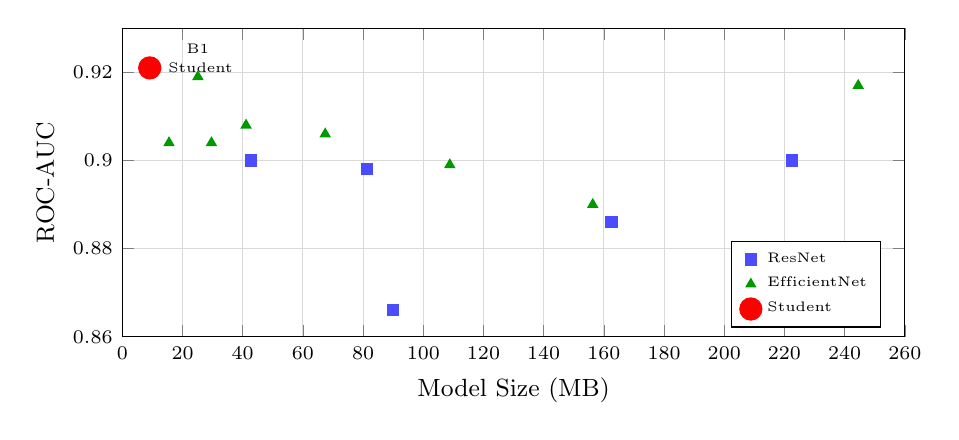
\begin{tikzpicture}
\begin{axis}[
    width=0.95\columnwidth,
    height=5.5cm,
    xlabel={Model Size (MB)},
    ylabel={ROC-AUC},
    xmin=0, xmax=260,
    ymin=0.86, ymax=0.93,
    legend pos=south east,
    legend style={font=\tiny, cells={anchor=west}},
    grid=major,
    grid style={gray!30},
    tick label style={font=\scriptsize},
    label style={font=\small},
    scatter/classes={
        resnet={mark=square*, blue!70},
        efficient={mark=triangle*, green!60!black},
        student={mark=*, red, mark size=4pt}
    },
]
% ResNet models
\addplot[scatter, only marks, scatter src=explicit symbolic]
coordinates {
    (42.7, 0.900) [resnet]
    (81.3, 0.898) [resnet]
    (89.9, 0.866) [resnet]
    (162.5, 0.886) [resnet]
    (222.4, 0.900) [resnet]
};
% EfficientNet models
\addplot[scatter, only marks, scatter src=explicit symbolic]
coordinates {
    (15.5, 0.904) [efficient]
    (25.1, 0.919) [efficient]
    (29.6, 0.904) [efficient]
    (41.1, 0.908) [efficient]
    (67.4, 0.906) [efficient]
    (108.8, 0.899) [efficient]
    (156.3, 0.890) [efficient]
    (244.5, 0.917) [efficient]
};
% Student model (highlighted)
\addplot[scatter, only marks, scatter src=explicit symbolic]
coordinates {
    (9.1, 0.921) [student]
};

% Annotations
\node[font=\tiny, anchor=west] at (axis cs:12, 0.921) {Student};
\node[font=\tiny, anchor=south] at (axis cs:25.1, 0.922) {B1};

\legend{ResNet, EfficientNet, Student}
\end{axis}
\end{tikzpicture}
\caption{Model size vs. ROC-AUC trade-off. The distilled student (red circle) achieves the highest ROC-AUC with the smallest model size, demonstrating effective knowledge transfer.}
\label{fig:model_comparison}
\end{figure}

\begin{table}[t]
\centering
\caption{Deployment comparison: teacher vs. student.}
\label{tab:deployment}
\begin{tabular}{lccc}
\toprule
\textbf{Model} & \textbf{Size (MB)} & \textbf{Latency (ms)} & \textbf{ROC-AUC} \\
\midrule
EfficientNet-B1 (Teacher) & 25.1 & 8.6 & 0.919 \\
MobileNetV3-Small (Student) & 9.1 & $\sim$3 & \textbf{0.921} \\
\midrule
\textbf{Compression Ratio} & \textbf{2.8$\times$} & \textbf{2.9$\times$} & +0.002 \\
\bottomrule
\end{tabular}
\end{table}

Fig.~\ref{fig:latency} compares inference latency across all models, highlighting the student's efficiency advantage for mobile deployment.

\begin{figure}[t]
\centering
\begin{tikzpicture}
\begin{axis}[
    width=0.95\columnwidth,
    height=5cm,
    xbar,
    xlabel={CPU Latency (ms)},
    symbolic y coords={Student, B0, B1, B2, B3, B4, B5, B6, B7, R-18, R-34, R-50, R-101, R-152},
    ytick=data,
    y tick label style={font=\tiny},
    xmin=0, xmax=25,
    nodes near coords,
    nodes near coords align={horizontal},
    nodes near coords style={font=\tiny},
    bar width=6pt,
    tick label style={font=\scriptsize},
    label style={font=\small},
    legend pos=south east,
    legend style={font=\tiny},
]
\addplot[fill=red!60, draw=red!80] coordinates {
    (3, Student)
};
\addplot[fill=green!50, draw=green!70] coordinates {
    (6.0, B0) (8.6, B1) (8.9, B2) (9.7, B3) (11.9, B4) (14.8, B5) (17.2, B6) (20.4, B7)
};
\addplot[fill=blue!50, draw=blue!70] coordinates {
    (1.9, R-18) (3.4, R-34) (4.9, R-50) (9.0, R-101) (14.4, R-152)
};
\legend{Student, EfficientNet, ResNet}
\end{axis}
\end{tikzpicture}
\caption{CPU inference latency comparison. The student (red) achieves competitive latency while matching EfficientNet accuracy. ResNet models are faster but less accurate.}
\label{fig:latency}
\end{figure}

\subsection{Error Analysis}

On the holdout set (1,513 images, 172 melanoma positive, 11.4\% prevalence):

\begin{table}[t]
\centering
\caption{Teacher vs. student agreement analysis on holdout set.}
\label{tab:agreement}
\begin{tabular}{lcc}
\toprule
\textbf{Metric} & \textbf{Count} & \textbf{Percentage} \\
\midrule
Total samples & 1,513 & 100\% \\
Models agree & 1,331 & 88.0\% \\
Models disagree & 182 & 12.0\% \\
\midrule
Teacher correct & 1,307 & 86.4\% \\
Student correct & 1,369 & 90.5\% \\
Both correct & 1,247 & 82.4\% \\
Both wrong & 84 & 5.6\% \\
\midrule
Shared false negatives & 29 & 16.9\% of melanomas \\
Shared false positives & 55 & 4.1\% of benign \\
\bottomrule
\end{tabular}
\end{table}

Table~\ref{tab:agreement} summarizes model agreement. Key findings:

\begin{itemize}
    \item When models disagree (182 cases), the student is correct 67\% of the time (122 vs 60 cases)
    \item 29 shared false negatives represent challenging melanomas with atypical features that neither model detects
    \item The student's higher accuracy (90.5\% vs 86.4\%) suggests effective regularization from soft labels
\end{itemize}

The shared false negatives represent challenging lesions with atypical features, suggesting the need for ensemble approaches or additional training data for edge cases.

%============================================================================
% 5. DISCUSSION AND FUTURE WORK
%============================================================================
\section{Discussion and Future Work}

\subsection{Planned Improvements}

\begin{enumerate}
    \item \textbf{Quantization-Aware Training:} If INT8 post-training quantization degrades performance substantially, we will implement QAT to recover accuracy while targeting $<$2 MB for edge deployment.
    
    \item \textbf{Multi-Teacher Distillation:} Ensemble soft labels from multiple teachers (e.g., EfficientNet-B1 + B2 + B3) may improve student calibration and reduce shared failure cases.
    
    \item \textbf{Feature-Based Distillation:} Beyond logit matching, intermediate feature distillation \cite{romero2014fitnets} may transfer richer representations.
    
    \item \textbf{Mobile Deployment Testing:} Profile inference on actual iOS/Android devices using CoreML/TensorFlow Lite to validate latency estimates.
    
    \item \textbf{Extended Evaluation:} Test on external dermoscopy datasets (ISIC 2019/2020, PH$^2$) to assess generalization.
\end{enumerate}

\subsection{Clinical Considerations}

Our model should be viewed as a high-sensitivity decision-support and pre-screening tool, not a stand-alone diagnostic application \cite{papachristou2024evaluation,jahn2022overdetection,smakgregoor2023ai}. This distinction is critical for appropriate clinical deployment.

\textbf{Sensitivity-Specificity Trade-off:} Prior primary care and mobile app studies demonstrate that prioritizing sensitivity and negative predictive value minimizes false negatives (missed melanomas) but inevitably increases false positives \cite{papachristou2024evaluation,jahn2022overdetection}. Our model achieves 75\% sensitivity at 92.5\% specificity, but clinical deployment may require adjusting this threshold based on the specific use case and acceptable referral rates.

\textbf{Intended Use Setting:} Because our model was trained exclusively on dermoscopic images, its use should be limited to settings where similar dermoscopic photos are available (e.g., primary care with dermatoscopes, teledermatology platforms). Performance is expected to degrade significantly on casual smartphone photos taken at home without standardized lighting or magnification \cite{papachristou2024evaluation,behara2024ai,smakgregoor2023ai}.

\textbf{Demographic Bias and Equity:} Most publicly available dermoscopy datasets, including HAM10000, over-represent lighter skin types (Fitzpatrick I--III) \cite{behara2024ai,salinas2024systematic}. Generalizability to darker skin tones remains uncertain and requires explicit validation before deployment in diverse populations. This is a critical equity concern that must be addressed through dataset diversification and prospective validation studies.

\textbf{Health System Impact:} Any deployment must consider downstream effects on healthcare systems, including monitoring impacts on referral patterns, biopsy rates, and costs to avoid unintended overuse of specialist services \cite{papachristou2024evaluation,smakgregoor2023ai}. A high false-positive rate, while acceptable for individual patient safety, may strain dermatology resources if deployed at scale.

\textbf{Appropriate Clinical Role:} Our model is best used to flag suspicious lesions for clinician review rather than to reassure patients that a lesion is benign \cite{jahn2022overdetection,smakgregoor2023ai}. The model should augment, not replace, clinical judgment, and patients should be counseled that negative results do not eliminate the need for professional evaluation of concerning lesions.

\subsection{Limitations}

This study has several limitations that should be acknowledged:

\begin{itemize}
    \item \textbf{Single dataset:} Evaluation is limited to HAM10000; generalization to other dermoscopy datasets (ISIC 2019/2020, PH$^2$) or clinical settings remains to be validated \cite{salinas2024systematic}
    
    \item \textbf{Dermoscopic images only:} Our model is trained on professional dermoscopic images with standardized acquisition protocols; performance on casual smartphone photos without dermatoscope attachments is expected to be substantially lower \cite{papachristou2024evaluation,behara2024ai}
    
    \item \textbf{Binary classification:} We simplify the seven-class diagnostic problem to melanoma vs. non-melanoma, potentially missing clinically-relevant distinctions among benign lesion types
    
    \item \textbf{Limited hyperparameter search:} Due to computational constraints, we explored only $T \in \{1, 2\}$ and $\alpha \in \{0.5, 0.9\}$; finer-grained search may yield better configurations
    
    \item \textbf{Demographic representation:} HAM10000 over-represents lighter skin types (Fitzpatrick I--III), limiting generalizability to diverse populations \cite{behara2024ai,salinas2024systematic}
    
    \item \textbf{No prospective validation:} Our evaluation is retrospective on held-out data; prospective clinical trials are needed to assess real-world performance and integration into clinical workflows \cite{papachristou2024evaluation}
    
    \item \textbf{No real-device testing:} Latency estimates are based on CPU inference benchmarks; actual mobile performance depends on device-specific hardware and software optimizations
\end{itemize}

%============================================================================
% 6. MEMBER CONTRIBUTIONS
%============================================================================
\section{Member Contributions}

\textbf{Ryan Healy:} Project infrastructure and codebase development, data pipeline implementation with lesion-aware splitting, teacher model training and evaluation (ResNet and EfficientNet families), knowledge distillation implementation and ablation studies, model quantization experiments, Weights \& Biases integration for experiment tracking, and paper writing.

\textbf{Heejeong (Angie) Yoon:} Literature review and related work analysis, traditional ML baseline experiments (Random Forest, SVM, Gradient Boosting), data augmentation strategy design, calibration analysis and reliability diagram implementation, clinical deployment considerations, error analysis, and paper writing and editing.

%============================================================================
% 7. CONCLUSION
%============================================================================
\section{Conclusion}

We presented a knowledge distillation framework for melanoma detection that achieves state-of-the-art performance on HAM10000 while meeting mobile deployment constraints. Our MobileNetV3-Small student (9.1 MB) achieves ROC-AUC 0.921, exceeding all 13 teacher models while being 2.8$\times$ smaller and 2.9$\times$ faster than the best teacher. Key findings include: (1) lower distillation temperatures ($T=1$) outperform higher values commonly used in the literature; (2) balanced soft/hard label weighting ($\alpha=0.5$) yields optimal discrimination; and (3) rigorous lesion-aware data splitting is essential for realistic performance estimates. Future work will focus on quantization-aware training for edge deployment and validation on external datasets.

\section*{Acknowledgment}

The authors thank the DS 6050 Deep Learning course staff at the University of Virginia for guidance and feedback throughout this project.

%============================================================================
% REFERENCES
%============================================================================
\bibliographystyle{IEEEtran}
\begin{thebibliography}{22}

\bibitem{siegel2023cancer}
R.~L. Siegel, K.~D. Miller, N.~S. Wagle, and A. Jemal, ``Cancer statistics, 2023,'' \emph{CA: A Cancer Journal for Clinicians}, vol.~73, no.~1, pp.~17--48, 2023.

\bibitem{american_cancer_society_2024}
American Cancer Society, ``Cancer Facts \& Figures 2024,'' Atlanta: American Cancer Society, 2024.

\bibitem{esteva2017dermatologist}
A. Esteva \emph{et~al.}, ``Dermatologist-level classification of skin cancer with deep neural networks,'' \emph{Nature}, vol.~542, no.~7639, pp.~115--118, 2017.

\bibitem{haenssle2018man}
H.~A. Haenssle \emph{et~al.}, ``Man against machine: Diagnostic performance of a deep learning convolutional neural network for dermoscopic melanoma recognition in comparison to 58 dermatologists,'' \emph{Annals of Oncology}, vol.~29, no.~8, pp.~1836--1842, 2018.

\bibitem{hinton2015distilling}
G. Hinton, O. Vinyals, and J. Dean, ``Distilling the knowledge in a neural network,'' \emph{arXiv preprint arXiv:1503.02531}, 2015.

\bibitem{tschandl2018ham10000}
P. Tschandl, C. Rosendahl, and H. Kittler, ``The HAM10000 dataset, a large collection of multi-source dermatoscopic images of common pigmented skin lesions,'' \emph{Scientific Data}, vol.~5, p.~180161, 2018.

\bibitem{he2016deep}
K. He, X. Zhang, S. Ren, and J. Sun, ``Deep residual learning for image recognition,'' in \emph{Proc. IEEE Conf. Computer Vision and Pattern Recognition (CVPR)}, 2016, pp.~770--778.

\bibitem{tan2019efficientnet}
M. Tan and Q. Le, ``EfficientNet: Rethinking model scaling for convolutional neural networks,'' in \emph{Proc. Int. Conf. Machine Learning (ICML)}, 2019, pp.~6105--6114.

\bibitem{islam2022knowledge}
M.~T. Islam, M.~A. Aowal, A.~T. Minhaz, and K. Ashraf, ``Knowledge distillation for skin lesion classification,'' in \emph{MICCAI Workshop on Medical Image Learning with Limited and Noisy Data}, 2022.

\bibitem{kabir2021spinenet}
H.~M.~D. Kabir \emph{et~al.}, ``SpineNet: Automated classification and evidence visualization in spinal MRIs,'' \emph{Medical Image Analysis}, vol.~71, p.~102054, 2021.

\bibitem{nazari2023multi}
P. Nazari and E.~B. Kovacs, ``Multi-teacher knowledge distillation for histopathology image classification,'' \emph{IEEE Journal of Biomedical and Health Informatics}, vol.~27, no.~5, 2023.

\bibitem{polino2018model}
A. Polino, R. Pascanu, and D. Alistarh, ``Model compression via distillation and quantization,'' in \emph{Proc. Int. Conf. Learning Representations (ICLR)}, 2018.

\bibitem{gou2021knowledge}
J. Gou, B. Yu, S.~J. Maybank, and D. Tao, ``Knowledge distillation: A survey,'' \emph{International Journal of Computer Vision}, vol.~129, no.~6, pp.~1789--1819, 2021.

\bibitem{howard2019searching}
A. Howard \emph{et~al.}, ``Searching for MobileNetV3,'' in \emph{Proc. IEEE/CVF Int. Conf. Computer Vision (ICCV)}, 2019, pp.~1314--1324.

\bibitem{lin2017focal}
T.-Y. Lin, P. Goyal, R. Girshick, K. He, and P. Doll\'{a}r, ``Focal loss for dense object detection,'' in \emph{Proc. IEEE Int. Conf. Computer Vision (ICCV)}, 2017, pp.~2980--2988.

\bibitem{loshchilov2017decoupled}
I. Loshchilov and F. Hutter, ``Decoupled weight decay regularization,'' in \emph{Proc. Int. Conf. Learning Representations (ICLR)}, 2019.

\bibitem{romero2014fitnets}
A. Romero, N. Ballas, S.~E. Kahou, A. Chassang, C. Gatta, and Y. Bengio, ``FitNets: Hints for thin deep nets,'' in \emph{Proc. Int. Conf. Learning Representations (ICLR)}, 2015.

\bibitem{papachristou2024evaluation}
P. Papachristou \emph{et~al.}, ``Evaluation of an artificial intelligence-based decision support for the detection of cutaneous melanoma in primary care: a prospective real-life clinical trial,'' \emph{British Journal of Dermatology}, vol.~191, no.~1, pp.~125--133, 2024.

\bibitem{jahn2022overdetection}
A.~S. Jahn \emph{et~al.}, ``Over-detection of melanoma-suspect lesions by a CE-certified smartphone app: Performance in comparison to dermatologists, 2D and 3D convolutional neural networks,'' \emph{Cancers}, vol.~14, no.~15, art.~3829, 2022.

\bibitem{behara2024ai}
K. Behara, E. Bhero, and J.~T. Agee, ``AI in dermatology: A comprehensive review into skin cancer detection,'' \emph{PeerJ Computer Science}, vol.~10, art.~e2530, 2024.

\bibitem{salinas2024systematic}
M.~P. Salinas \emph{et~al.}, ``A systematic review and meta-analysis of artificial intelligence versus clinicians for skin cancer diagnosis,'' \emph{npj Digital Medicine}, vol.~7, no.~1, art.~125, 2024.

\bibitem{smakgregoor2023ai}
A.~M. Smak~Gregoor \emph{et~al.}, ``An artificial intelligence based app for skin cancer detection evaluated in a population based setting,'' \emph{npj Digital Medicine}, vol.~6, no.~1, art.~90, 2023.

\end{thebibliography}

\end{document}
